% Page: Joint distributions
% sources/stat2003/chapters/prob-04-joint-distributions.qmd
% The construction in "A point in a triangle": X uniform on [0,1],
% then Y uniform on [0,X]. The support is the triangle with vertices
% (0,0), (1,0) and (1,1). The conditional distribution is the vertical slice.
\documentclass[border=6pt]{standalone}
\usepackage[T1]{fontenc}
\usepackage{lmodern}
\usepackage{amsmath,amssymb}
\usepackage{tikz}
\usepackage{pgfplots}
\pgfplotsset{compat=1.18}
\definecolor{ink}{HTML}{1F2430}
\definecolor{statblue}{HTML}{174A7E}
\definecolor{bluefill}{HTML}{D7E5F0}
\definecolor{accent}{HTML}{9C4A32}
\definecolor{grey}{HTML}{5E6A75}
\pgfplotsset{
  stat/.style={
    scale only axis,
    axis lines=left,
    axis line style={ink, line width=0.6pt},
    tick style={ink, line width=0.45pt},
    tick label style={font=\small, text=ink},
    label style={font=\small, text=ink},
    title style={font=\small, text=ink, align=center},
    clip=false,
    unbounded coords=jump,
    scaled ticks=false,
  },
}
\begin{document}
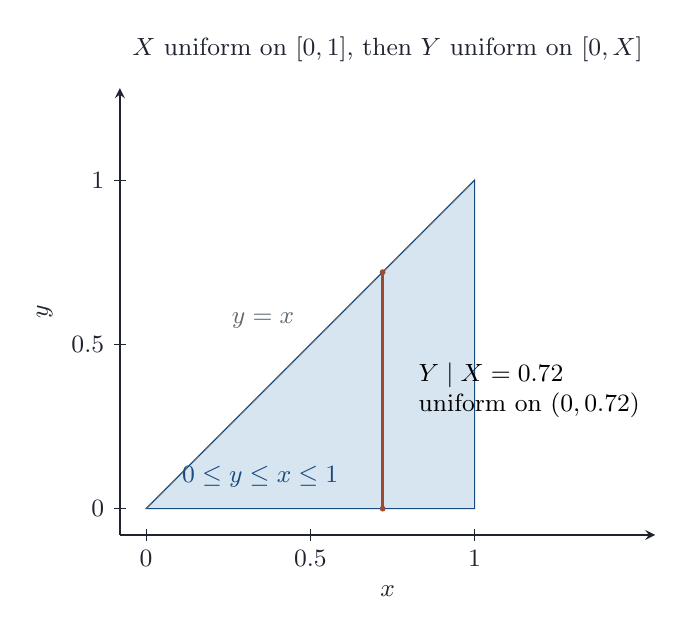
\begin{tikzpicture}
\begin{axis}[
  stat, width=6.8cm, height=6.8cm,
  xmin=-0.08, xmax=1.55, ymin=-0.08, ymax=1.28,
  xtick={0,0.5,1},
  ytick={0,0.5,1},
  xlabel={$x$},
  ylabel={$y$},
  axis equal image,
  title={$X$ uniform on $[0,1]$, then $Y$ uniform on $[0,X]$},
]
  \fill[bluefill] (axis cs:0,0) -- (axis cs:1,0) -- (axis cs:1,1) -- cycle;
  \draw[statblue, thin] (axis cs:0,0) -- (axis cs:1,0) -- (axis cs:1,1) -- cycle;
  \draw[grey, dashed, thin] (axis cs:0,0) -- (axis cs:1,1);
  \draw[accent, line width=1.15pt] (axis cs:0.72,0) -- (axis cs:0.72,0.72);
  \fill[accent] (axis cs:0.72,0) circle[radius=1.05pt];
  \fill[accent] (axis cs:0.72,0.72) circle[radius=1.05pt];
  \node[font=\small, anchor=south east, grey] at (axis cs:0.48,0.52) {$y=x$};
  \node[font=\small, align=left, anchor=west] at (axis cs:0.80,0.36)
    {$Y\mid X=0.72$\\uniform on $(0,0.72)$};
  \node[font=\small, statblue, anchor=north west] at (axis cs:0.08,0.16)
    {$0\le y\le x\le 1$};
\end{axis}
\end{tikzpicture}
\end{document}
